\documentclass{article}
\usepackage[utf8]{inputenc}
\usepackage{graphicx}
\usepackage{listings}
\title{Information System - Lab work 9}
\author{Tran Thi Hong Hanh}
\date{10 November 2017}

\begin{document}

\maketitle
\section*{Database}

\begin{itemize}
	\item Which normal form does the employee database sastisfy?\\
Employee database has information stored in relational database with each column containing atomic value and no repeated columns. 
On the other hand, each non-key column depends on primary keys. And there are no columns that are non-transitively dependent on the primary key and you can infer information from other table using foreign keys. Hence, the database also satisfies Third Normal Form (3NF).

\end{itemize}

\section*{Normalization}
\begin{itemize}
	\item Produce a 3NF of the following Order form document by normalization.
\begin{figure}[h]
\centering
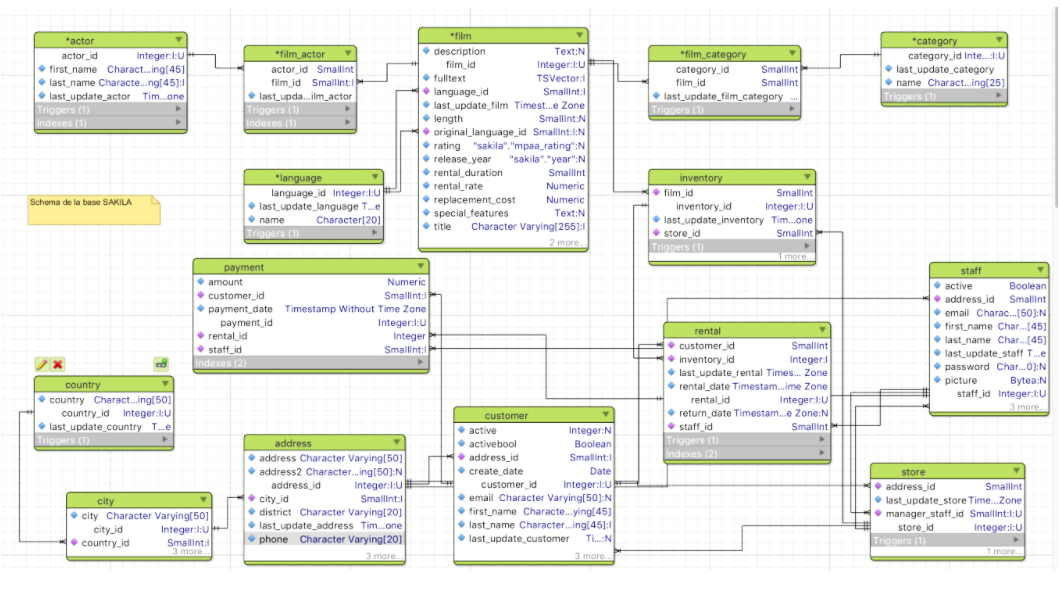
\includegraphics[scale = 0.5]{schema.PNG}
\caption{Databases}
\end{figure}
\end{itemize}
\end{document}
